% Options for packages loaded elsewhere
\PassOptionsToPackage{unicode}{hyperref}
\PassOptionsToPackage{hyphens}{url}
\PassOptionsToPackage{dvipsnames,svgnames,x11names}{xcolor}
%
\documentclass[
]{agujournal2019}

\usepackage{amsmath,amssymb}
\usepackage{iftex}
\ifPDFTeX
  \usepackage[T1]{fontenc}
  \usepackage[utf8]{inputenc}
  \usepackage{textcomp} % provide euro and other symbols
\else % if luatex or xetex
  \usepackage{unicode-math}
  \defaultfontfeatures{Scale=MatchLowercase}
  \defaultfontfeatures[\rmfamily]{Ligatures=TeX,Scale=1}
\fi
\usepackage{lmodern}
\ifPDFTeX\else  
    % xetex/luatex font selection
\fi
% Use upquote if available, for straight quotes in verbatim environments
\IfFileExists{upquote.sty}{\usepackage{upquote}}{}
\IfFileExists{microtype.sty}{% use microtype if available
  \usepackage[]{microtype}
  \UseMicrotypeSet[protrusion]{basicmath} % disable protrusion for tt fonts
}{}
\makeatletter
\@ifundefined{KOMAClassName}{% if non-KOMA class
  \IfFileExists{parskip.sty}{%
    \usepackage{parskip}
  }{% else
    \setlength{\parindent}{0pt}
    \setlength{\parskip}{6pt plus 2pt minus 1pt}}
}{% if KOMA class
  \KOMAoptions{parskip=half}}
\makeatother
\usepackage{xcolor}
\setlength{\emergencystretch}{3em} % prevent overfull lines
\setcounter{secnumdepth}{5}
% Make \paragraph and \subparagraph free-standing
\ifx\paragraph\undefined\else
  \let\oldparagraph\paragraph
  \renewcommand{\paragraph}[1]{\oldparagraph{#1}\mbox{}}
\fi
\ifx\subparagraph\undefined\else
  \let\oldsubparagraph\subparagraph
  \renewcommand{\subparagraph}[1]{\oldsubparagraph{#1}\mbox{}}
\fi


\providecommand{\tightlist}{%
  \setlength{\itemsep}{0pt}\setlength{\parskip}{0pt}}\usepackage{longtable,booktabs,array}
\usepackage{calc} % for calculating minipage widths
% Correct order of tables after \paragraph or \subparagraph
\usepackage{etoolbox}
\makeatletter
\patchcmd\longtable{\par}{\if@noskipsec\mbox{}\fi\par}{}{}
\makeatother
% Allow footnotes in longtable head/foot
\IfFileExists{footnotehyper.sty}{\usepackage{footnotehyper}}{\usepackage{footnote}}
\makesavenoteenv{longtable}
\usepackage{graphicx}
\makeatletter
\def\maxwidth{\ifdim\Gin@nat@width>\linewidth\linewidth\else\Gin@nat@width\fi}
\def\maxheight{\ifdim\Gin@nat@height>\textheight\textheight\else\Gin@nat@height\fi}
\makeatother
% Scale images if necessary, so that they will not overflow the page
% margins by default, and it is still possible to overwrite the defaults
% using explicit options in \includegraphics[width, height, ...]{}
\setkeys{Gin}{width=\maxwidth,height=\maxheight,keepaspectratio}
% Set default figure placement to htbp
\makeatletter
\def\fps@figure{htbp}
\makeatother
% definitions for citeproc citations
\NewDocumentCommand\citeproctext{}{}
\NewDocumentCommand\citeproc{mm}{%
  \begingroup\def\citeproctext{#2}\cite{#1}\endgroup}
\makeatletter
 % allow citations to break across lines
 \let\@cite@ofmt\@firstofone
 % avoid brackets around text for \cite:
 \def\@biblabel#1{}
 \def\@cite#1#2{{#1\if@tempswa , #2\fi}}
\makeatother
\newlength{\cslhangindent}
\setlength{\cslhangindent}{1.5em}
\newlength{\csllabelwidth}
\setlength{\csllabelwidth}{3em}
\newenvironment{CSLReferences}[2] % #1 hanging-indent, #2 entry-spacing
 {\begin{list}{}{%
  \setlength{\itemindent}{0pt}
  \setlength{\leftmargin}{0pt}
  \setlength{\parsep}{0pt}
  % turn on hanging indent if param 1 is 1
  \ifodd #1
   \setlength{\leftmargin}{\cslhangindent}
   \setlength{\itemindent}{-1\cslhangindent}
  \fi
  % set entry spacing
  \setlength{\itemsep}{#2\baselineskip}}}
 {\end{list}}
\usepackage{calc}
\newcommand{\CSLBlock}[1]{\hfill\break\parbox[t]{\linewidth}{\strut\ignorespaces#1\strut}}
\newcommand{\CSLLeftMargin}[1]{\parbox[t]{\csllabelwidth}{\strut#1\strut}}
\newcommand{\CSLRightInline}[1]{\parbox[t]{\linewidth - \csllabelwidth}{\strut#1\strut}}
\newcommand{\CSLIndent}[1]{\hspace{\cslhangindent}#1}

\usepackage{booktabs}
\usepackage{longtable}
\usepackage{array}
\usepackage{multirow}
\usepackage{wrapfig}
\usepackage{float}
\usepackage{colortbl}
\usepackage{pdflscape}
\usepackage{tabu}
\usepackage{threeparttable}
\usepackage{threeparttablex}
\usepackage[normalem]{ulem}
\usepackage{makecell}
\usepackage{xcolor}
\usepackage{caption}
\usepackage{graphicx}
\usepackage{siunitx}
\usepackage{hhline}
\usepackage{calc}
\usepackage{tabularx}
\usepackage{adjustbox}
\usepackage{hyperref}
\usepackage{url} %this package should fix any errors with URLs in refs.
\usepackage{lineno}
\usepackage[inline]{trackchanges} %for better track changes. finalnew option will compile document with changes incorporated.
\usepackage{soul}
\linenumbers
\makeatletter
\@ifpackageloaded{tcolorbox}{}{\usepackage[skins,breakable]{tcolorbox}}
\@ifpackageloaded{fontawesome5}{}{\usepackage{fontawesome5}}
\definecolor{quarto-callout-color}{HTML}{909090}
\definecolor{quarto-callout-note-color}{HTML}{0758E5}
\definecolor{quarto-callout-important-color}{HTML}{CC1914}
\definecolor{quarto-callout-warning-color}{HTML}{EB9113}
\definecolor{quarto-callout-tip-color}{HTML}{00A047}
\definecolor{quarto-callout-caution-color}{HTML}{FC5300}
\definecolor{quarto-callout-color-frame}{HTML}{acacac}
\definecolor{quarto-callout-note-color-frame}{HTML}{4582ec}
\definecolor{quarto-callout-important-color-frame}{HTML}{d9534f}
\definecolor{quarto-callout-warning-color-frame}{HTML}{f0ad4e}
\definecolor{quarto-callout-tip-color-frame}{HTML}{02b875}
\definecolor{quarto-callout-caution-color-frame}{HTML}{fd7e14}
\makeatother
\makeatletter
\@ifpackageloaded{caption}{}{\usepackage{caption}}
\AtBeginDocument{%
\ifdefined\contentsname
  \renewcommand*\contentsname{Table of contents}
\else
  \newcommand\contentsname{Table of contents}
\fi
\ifdefined\listfigurename
  \renewcommand*\listfigurename{List of Figures}
\else
  \newcommand\listfigurename{List of Figures}
\fi
\ifdefined\listtablename
  \renewcommand*\listtablename{List of Tables}
\else
  \newcommand\listtablename{List of Tables}
\fi
\ifdefined\figurename
  \renewcommand*\figurename{Figure}
\else
  \newcommand\figurename{Figure}
\fi
\ifdefined\tablename
  \renewcommand*\tablename{Table}
\else
  \newcommand\tablename{Table}
\fi
}
\@ifpackageloaded{float}{}{\usepackage{float}}
\floatstyle{ruled}
\@ifundefined{c@chapter}{\newfloat{codelisting}{h}{lop}}{\newfloat{codelisting}{h}{lop}[chapter]}
\floatname{codelisting}{Listing}
\newcommand*\listoflistings{\listof{codelisting}{List of Listings}}
\makeatother
\makeatletter
\makeatother
\makeatletter
\@ifpackageloaded{caption}{}{\usepackage{caption}}
\@ifpackageloaded{subcaption}{}{\usepackage{subcaption}}
\makeatother
\ifLuaTeX
  \usepackage{selnolig}  % disable illegal ligatures
\fi
\usepackage{bookmark}

\IfFileExists{xurl.sty}{\usepackage{xurl}}{} % add URL line breaks if available
\urlstyle{same} % disable monospaced font for URLs
\hypersetup{
  pdftitle={Linearity for Tranduction Efficiency Assay Qualification},
  colorlinks=true,
  linkcolor={blue},
  filecolor={Maroon},
  citecolor={Blue},
  urlcolor={Blue},
  pdfcreator={LaTeX via pandoc}}


\draftfalse

\begin{document}
\title{Linearity for Tranduction Efficiency Assay Qualification}

\authors{Adeline Chew\affil{1}, Yu Xin Lim\affil{1}, Jinkai
Teo\affil{1}}
\affiliation{1}{Tikva Allocell Pte. Ltd., }
\correspondingauthor{Jinkai Teo}{jinkaiteo@tikvaallocell.com}






\section{Introduction}\label{introduction}

This report documents the statistical analysis performed for the
linearity of the Transduction Efficiency (TE) Assay. This document is
intended to be read as part of the qualification report for Tranduction
Efficiency. In brief, the TE assay employs a flow cytometry method to
establish the proportion of transduced cells in the test article (cell
suspension). In the manufacturing of the CART cells, B7-H3 and Serpin B9
(CAS) were introduced into the T cells via transduction using a
replication-incompetent retrovirus vector. Fluorescent-labeled
antibodies targeting the VHH and T2A were used to label the B7-H3.CAR
and the transduced Serpin B9 (CAS). The proportion of the positively
stained cells (B7-H3 and Serpin B9 (CAS) positive) out of the total
amount of cells in the cell suspension is reported as the Transduction
Efficiency.

\textsubscript{Source:
\href{https://jinkaiteo.github.io/quarto-template/index.qmd.html}{Article
Notebook}}

\section{Data generated for
Linearity}\label{data-generated-for-linearity}

The IHC harmonized tripartite guideline (Borman \& Elder, 2017) defines
linearity as:

\begin{tcolorbox}[enhanced jigsaw, coltitle=black, breakable, opacitybacktitle=0.6, colbacktitle=quarto-callout-note-color!10!white, toprule=.15mm, opacityback=0, bottomtitle=1mm, titlerule=0mm, colframe=quarto-callout-note-color-frame, leftrule=.75mm, title=\textcolor{quarto-callout-note-color}{\faInfo}\hspace{0.5em}{IHC Guidlines}, toptitle=1mm, colback=white, arc=.35mm, rightrule=.15mm, bottomrule=.15mm, left=2mm]

A linear relationship should be evaluated across the range of the
analytical procedure. It may be demonstrated directly on the drug
substance (by dilution of a standard stock solution) and/or separate
weighings of synthetic mixtures of the drug product components, using
the proposed procedure. The latter aspect can be studied during
investigation of the range.

\end{tcolorbox}

In line with this guidance, samples with different transduction
efficient were generated using CART cells expressing the B7-H3 CAR
antigen (drug substance, DS) are diluted at various known ration (volume
per volume) with untransduced T cells that does not express the CAR on
the surface, as shown in Table~\ref{tbl-rawdata}. The expected
transduction efficiency was normalized based on the 100\%(v/v) and 0
\%(v/v). These set of samples were ran by two operators across three
days to incorporate inter-operator and inter-day variations.

\textsubscript{Source:
\href{https://jinkaiteo.github.io/quarto-template/index.qmd.html}{Article
Notebook}}

\begin{table}

\caption{\label{tbl-rawdata}Data generated for linearity in
qualification}

\centering{

\centering
\begin{tabular}[t]{c|c|c|c}
\hline
Operator & Day & Observed (\%TE) & Expected (\%TE)\\
\hline
 &  & 0.00 & 0.00\\
\cline{3-4}
 &  & 16.85 & 16.91\\
\cline{3-4}
 &  & 33.49 & 33.82\\
\cline{3-4}
 &  & 52.28 & 50.73\\
\cline{3-4}
 &  & 69.70 & 67.64\\
\cline{3-4}
 & \multirow{-6}{*}{\centering\arraybackslash Day1} & 83.62 & 84.55\\
\cline{2-4}
 &  & 0.00 & 0.00\\
\cline{3-4}
 &  & 14.81 & 16.91\\
\cline{3-4}
 &  & 33.33 & 33.82\\
\cline{3-4}
 &  & 51.54 & 50.73\\
\cline{3-4}
 &  & 67.39 & 67.64\\
\cline{3-4}
 & \multirow{-6}{*}{\centering\arraybackslash Day2} & 84.16 & 84.55\\
\cline{2-4}
 &  & 0.01 & 0.00\\
\cline{3-4}
 &  & 13.65 & 16.91\\
\cline{3-4}
 &  & 33.43 & 33.82\\
\cline{3-4}
 &  & 49.99 & 50.73\\
\cline{3-4}
 &  & 68.44 & 67.64\\
\cline{3-4}
\multirow{-18}{*}[1\dimexpr\aboverulesep+\belowrulesep+\cmidrulewidth]{\centering\arraybackslash Operator 1} & \multirow{-6}{*}{\centering\arraybackslash Day3} & 84.73 & 84.55\\
\cline{1-4}
 &  & 0.00 & 0.00\\
\cline{3-4}
 &  & 16.84 & 16.91\\
\cline{3-4}
 &  & 33.79 & 33.82\\
\cline{3-4}
 &  & 52.43 & 50.73\\
\cline{3-4}
 &  & 68.34 & 67.64\\
\cline{3-4}
 & \multirow{-6}{*}{\centering\arraybackslash Day1} & 84.26 & 84.55\\
\cline{2-4}
 &  & 0.00 & 0.00\\
\cline{3-4}
 &  & 14.94 & 16.91\\
\cline{3-4}
 &  & 32.43 & 33.82\\
\cline{3-4}
 &  & 50.61 & 50.73\\
\cline{3-4}
 &  & 68.26 & 67.64\\
\cline{3-4}
 & \multirow{-6}{*}{\centering\arraybackslash Day2} & 83.25 & 84.55\\
\cline{2-4}
 &  & 0.01 & 0.00\\
\cline{3-4}
 &  & 13.70 & 16.91\\
\cline{3-4}
 &  & 32.38 & 33.82\\
\cline{3-4}
 &  & 49.11 & 50.73\\
\cline{3-4}
 &  & 68.48 & 67.64\\
\cline{3-4}
\multirow{-18}{*}[1\dimexpr\aboverulesep+\belowrulesep+\cmidrulewidth]{\centering\arraybackslash Operator 2} & \multirow{-6}{*}{\centering\arraybackslash Day3} & 87.28 & 84.55\\
\hline
\end{tabular}

}

\end{table}%

\textsubscript{Source:
\href{https://jinkaiteo.github.io/quarto-template/index.qmd.html}{Article
Notebook}}

\section{Methods}\label{methods}

Taking reference to the IHC harmonized tripartite guideline (Borman \&
Elder, 2017):

\begin{tcolorbox}[enhanced jigsaw, coltitle=black, breakable, opacitybacktitle=0.6, colbacktitle=quarto-callout-note-color!10!white, toprule=.15mm, opacityback=0, bottomtitle=1mm, titlerule=0mm, colframe=quarto-callout-note-color-frame, leftrule=.75mm, title=\textcolor{quarto-callout-note-color}{\faInfo}\hspace{0.5em}{IHC Guidlines}, toptitle=1mm, colback=white, arc=.35mm, rightrule=.15mm, bottomrule=.15mm, left=2mm]

Linearity should be evaluated by visual inspection of a plot of signals
as a function of analyte concentration or content. If there is a linear
relationship, test results should be evaluated by appropriate
statistical methods, for example, by calculation of a regression line by
the method of least squares. In some cases, to obtain linearity between
assays and sample concentrations, the test data may need to be subjected
to a mathematical transformation prior to the regression analysis. Data
from the regression line itself may be helpful to provide mathematical
estimates of the degree of linearity.

The correlation coefficient, y-intercept, slope of the regression line
and residual sum of squares should be submitted. A plot of the data
should be included. In addition, an analysis of the deviation of the
actual data points from the regression line may also be helpful for
evaluating linearity.

\end{tcolorbox}

A similar method was employed in this analysis where a linear model is
used for the regression of the data collected within each operator
within the same day.

We used R version 4.3.2 (R Core Team, 2023) and the following R
packages: flextable v. 0.9.6 (Gohel \& Skintzos, 2024), huxtable v.
5.5.6 (Hugh-Jones, 2024), jtools v. 2.2.2 (Long, 2022), kableExtra v.
1.4.0 (Zhu, 2024), rmarkdown v. 2.25 (Allaire et al., 2023; Xie et al.,
2018, 2020), tidyverse v. 2.0.0 (Wickham et al., 2019), webshot2 v.
0.1.1 (Chang, 2023).

\textsubscript{Source:
\href{https://jinkaiteo.github.io/quarto-template/index.qmd.html}{Article
Notebook}}

\section{Results}\label{results}

\textsubscript{Source:
\href{https://jinkaiteo.github.io/quarto-template/index.qmd.html}{Article
Notebook}}

The y-intercept, slope and R2 are summarized in Table~\ref{tbl-reg},
while the sum of squares are summarized in Table~\ref{tbl-ss}.

\begin{table}

\caption{\label{tbl-reg}Regression parameters for linearity results}

\centering{

[ht]
\begin{centerbox}
\begin{threeparttable}
 \label{tab:tbl-reg}
\setlength{\tabcolsep}{0pt}
\begin{tabular}{l l l l l l l}


\hhline{>{\huxb{0, 0, 0}{0.8}}->{\huxb{0, 0, 0}{0.8}}->{\huxb{0, 0, 0}{0.8}}->{\huxb{0, 0, 0}{0.8}}->{\huxb{0, 0, 0}{0.8}}->{\huxb{0, 0, 0}{0.8}}->{\huxb{0, 0, 0}{0.8}}-}
\arrayrulecolor{black}

\multicolumn{1}{!{\huxvb{0, 0, 0}{0}}c!{\huxvb{0, 0, 0}{0}}}{\huxtpad{6pt + 1em}\centering \hspace{6pt}  \hspace{6pt}\huxbpad{6pt}} &
\multicolumn{1}{c!{\huxvb{0, 0, 0}{0}}}{\huxtpad{6pt + 1em}\centering \hspace{6pt} Operator 1, Day1 \hspace{6pt}\huxbpad{6pt}} &
\multicolumn{1}{c!{\huxvb{0, 0, 0}{0}}}{\huxtpad{6pt + 1em}\centering \hspace{6pt} Operator 1, Day2 \hspace{6pt}\huxbpad{6pt}} &
\multicolumn{1}{c!{\huxvb{0, 0, 0}{0}}}{\huxtpad{6pt + 1em}\centering \hspace{6pt} Operator 1, Day3 \hspace{6pt}\huxbpad{6pt}} &
\multicolumn{1}{c!{\huxvb{0, 0, 0}{0}}}{\huxtpad{6pt + 1em}\centering \hspace{6pt} Operator 2, Day1 \hspace{6pt}\huxbpad{6pt}} &
\multicolumn{1}{c!{\huxvb{0, 0, 0}{0}}}{\huxtpad{6pt + 1em}\centering \hspace{6pt} Operator 2, Day2 \hspace{6pt}\huxbpad{6pt}} &
\multicolumn{1}{c!{\huxvb{0, 0, 0}{0}}}{\huxtpad{6pt + 1em}\centering \hspace{6pt} Operator 2, Day3 \hspace{6pt}\huxbpad{6pt}} \tabularnewline[-0.5pt]


\hhline{>{\huxb{255, 255, 255}{0.4}}->{\huxb{0, 0, 0}{0.4}}->{\huxb{0, 0, 0}{0.4}}->{\huxb{0, 0, 0}{0.4}}->{\huxb{0, 0, 0}{0.4}}->{\huxb{0, 0, 0}{0.4}}->{\huxb{0, 0, 0}{0.4}}-}
\arrayrulecolor{black}

\multicolumn{1}{!{\huxvb{0, 0, 0}{0}}l!{\huxvb{0, 0, 0}{0}}}{\huxtpad{6pt + 1em}\raggedright \hspace{6pt} (Intercept) \hspace{6pt}\huxbpad{6pt}} &
\multicolumn{1}{r!{\huxvb{0, 0, 0}{0}}}{\huxtpad{6pt + 1em}\raggedleft \hspace{6pt} 0.12\hphantom{0}\hphantom{0}\hphantom{0}\hphantom{0} \hspace{6pt}\huxbpad{6pt}} &
\multicolumn{1}{r!{\huxvb{0, 0, 0}{0}}}{\huxtpad{6pt + 1em}\raggedleft \hspace{6pt} -0.76\hphantom{0}\hphantom{0}\hphantom{0}\hphantom{0} \hspace{6pt}\huxbpad{6pt}} &
\multicolumn{1}{r!{\huxvb{0, 0, 0}{0}}}{\huxtpad{6pt + 1em}\raggedleft \hspace{6pt} -1.47\hphantom{0}\hphantom{0}\hphantom{0}\hphantom{0} \hspace{6pt}\huxbpad{6pt}} &
\multicolumn{1}{r!{\huxvb{0, 0, 0}{0}}}{\huxtpad{6pt + 1em}\raggedleft \hspace{6pt} 0.15\hphantom{0}\hphantom{0}\hphantom{0}\hphantom{0} \hspace{6pt}\huxbpad{6pt}} &
\multicolumn{1}{r!{\huxvb{0, 0, 0}{0}}}{\huxtpad{6pt + 1em}\raggedleft \hspace{6pt} -0.88\hphantom{0}\hphantom{0}\hphantom{0}\hphantom{0} \hspace{6pt}\huxbpad{6pt}} &
\multicolumn{1}{r!{\huxvb{0, 0, 0}{0}}}{\huxtpad{6pt + 1em}\raggedleft \hspace{6pt} -2.28\hphantom{0}\hphantom{0}\hphantom{0}\hphantom{0} \hspace{6pt}\huxbpad{6pt}} \tabularnewline[-0.5pt]


\hhline{}
\arrayrulecolor{black}

\multicolumn{1}{!{\huxvb{0, 0, 0}{0}}l!{\huxvb{0, 0, 0}{0}}}{\huxtpad{6pt + 1em}\raggedright \hspace{6pt}  \hspace{6pt}\huxbpad{6pt}} &
\multicolumn{1}{r!{\huxvb{0, 0, 0}{0}}}{\huxtpad{6pt + 1em}\raggedleft \hspace{6pt} (0.93)\hphantom{0}\hphantom{0}\hphantom{0} \hspace{6pt}\huxbpad{6pt}} &
\multicolumn{1}{r!{\huxvb{0, 0, 0}{0}}}{\huxtpad{6pt + 1em}\raggedleft \hspace{6pt} (0.74)\hphantom{0}\hphantom{0}\hphantom{0} \hspace{6pt}\huxbpad{6pt}} &
\multicolumn{1}{r!{\huxvb{0, 0, 0}{0}}}{\huxtpad{6pt + 1em}\raggedleft \hspace{6pt} (1.01)\hphantom{0}\hphantom{0}\hphantom{0} \hspace{6pt}\huxbpad{6pt}} &
\multicolumn{1}{r!{\huxvb{0, 0, 0}{0}}}{\huxtpad{6pt + 1em}\raggedleft \hspace{6pt} (0.59)\hphantom{0}\hphantom{0}\hphantom{0} \hspace{6pt}\huxbpad{6pt}} &
\multicolumn{1}{r!{\huxvb{0, 0, 0}{0}}}{\huxtpad{6pt + 1em}\raggedleft \hspace{6pt} (0.80)\hphantom{0}\hphantom{0}\hphantom{0} \hspace{6pt}\huxbpad{6pt}} &
\multicolumn{1}{r!{\huxvb{0, 0, 0}{0}}}{\huxtpad{6pt + 1em}\raggedleft \hspace{6pt} (1.28)\hphantom{0}\hphantom{0}\hphantom{0} \hspace{6pt}\huxbpad{6pt}} \tabularnewline[-0.5pt]


\hhline{}
\arrayrulecolor{black}

\multicolumn{1}{!{\huxvb{0, 0, 0}{0}}l!{\huxvb{0, 0, 0}{0}}}{\huxtpad{6pt + 1em}\raggedright \hspace{6pt} Expected \hspace{6pt}\huxbpad{6pt}} &
\multicolumn{1}{r!{\huxvb{0, 0, 0}{0}}}{\huxtpad{6pt + 1em}\raggedleft \hspace{6pt} 1.01 *** \hspace{6pt}\huxbpad{6pt}} &
\multicolumn{1}{r!{\huxvb{0, 0, 0}{0}}}{\huxtpad{6pt + 1em}\raggedleft \hspace{6pt} 1.01 *** \hspace{6pt}\huxbpad{6pt}} &
\multicolumn{1}{r!{\huxvb{0, 0, 0}{0}}}{\huxtpad{6pt + 1em}\raggedleft \hspace{6pt} 1.02 *** \hspace{6pt}\huxbpad{6pt}} &
\multicolumn{1}{r!{\huxvb{0, 0, 0}{0}}}{\huxtpad{6pt + 1em}\raggedleft \hspace{6pt} 1.00 *** \hspace{6pt}\huxbpad{6pt}} &
\multicolumn{1}{r!{\huxvb{0, 0, 0}{0}}}{\huxtpad{6pt + 1em}\raggedleft \hspace{6pt} 1.00 *** \hspace{6pt}\huxbpad{6pt}} &
\multicolumn{1}{r!{\huxvb{0, 0, 0}{0}}}{\huxtpad{6pt + 1em}\raggedleft \hspace{6pt} 1.04 *** \hspace{6pt}\huxbpad{6pt}} \tabularnewline[-0.5pt]


\hhline{}
\arrayrulecolor{black}

\multicolumn{1}{!{\huxvb{0, 0, 0}{0}}l!{\huxvb{0, 0, 0}{0}}}{\huxtpad{6pt + 1em}\raggedright \hspace{6pt}  \hspace{6pt}\huxbpad{6pt}} &
\multicolumn{1}{r!{\huxvb{0, 0, 0}{0}}}{\huxtpad{6pt + 1em}\raggedleft \hspace{6pt} (0.02)\hphantom{0}\hphantom{0}\hphantom{0} \hspace{6pt}\huxbpad{6pt}} &
\multicolumn{1}{r!{\huxvb{0, 0, 0}{0}}}{\huxtpad{6pt + 1em}\raggedleft \hspace{6pt} (0.01)\hphantom{0}\hphantom{0}\hphantom{0} \hspace{6pt}\huxbpad{6pt}} &
\multicolumn{1}{r!{\huxvb{0, 0, 0}{0}}}{\huxtpad{6pt + 1em}\raggedleft \hspace{6pt} (0.02)\hphantom{0}\hphantom{0}\hphantom{0} \hspace{6pt}\huxbpad{6pt}} &
\multicolumn{1}{r!{\huxvb{0, 0, 0}{0}}}{\huxtpad{6pt + 1em}\raggedleft \hspace{6pt} (0.01)\hphantom{0}\hphantom{0}\hphantom{0} \hspace{6pt}\huxbpad{6pt}} &
\multicolumn{1}{r!{\huxvb{0, 0, 0}{0}}}{\huxtpad{6pt + 1em}\raggedleft \hspace{6pt} (0.02)\hphantom{0}\hphantom{0}\hphantom{0} \hspace{6pt}\huxbpad{6pt}} &
\multicolumn{1}{r!{\huxvb{0, 0, 0}{0}}}{\huxtpad{6pt + 1em}\raggedleft \hspace{6pt} (0.03)\hphantom{0}\hphantom{0}\hphantom{0} \hspace{6pt}\huxbpad{6pt}} \tabularnewline[-0.5pt]


\hhline{>{\huxb{255, 255, 255}{0.4}}->{\huxb{0, 0, 0}{0.4}}->{\huxb{0, 0, 0}{0.4}}->{\huxb{0, 0, 0}{0.4}}->{\huxb{0, 0, 0}{0.4}}->{\huxb{0, 0, 0}{0.4}}->{\huxb{0, 0, 0}{0.4}}-}
\arrayrulecolor{black}

\multicolumn{1}{!{\huxvb{0, 0, 0}{0}}l!{\huxvb{0, 0, 0}{0}}}{\huxtpad{6pt + 1em}\raggedright \hspace{6pt} N \hspace{6pt}\huxbpad{6pt}} &
\multicolumn{1}{r!{\huxvb{0, 0, 0}{0}}}{\huxtpad{6pt + 1em}\raggedleft \hspace{6pt} 6\hphantom{0}\hphantom{0}\hphantom{0}\hphantom{0}\hphantom{0}\hphantom{0}\hphantom{0} \hspace{6pt}\huxbpad{6pt}} &
\multicolumn{1}{r!{\huxvb{0, 0, 0}{0}}}{\huxtpad{6pt + 1em}\raggedleft \hspace{6pt} 6\hphantom{0}\hphantom{0}\hphantom{0}\hphantom{0}\hphantom{0}\hphantom{0}\hphantom{0} \hspace{6pt}\huxbpad{6pt}} &
\multicolumn{1}{r!{\huxvb{0, 0, 0}{0}}}{\huxtpad{6pt + 1em}\raggedleft \hspace{6pt} 6\hphantom{0}\hphantom{0}\hphantom{0}\hphantom{0}\hphantom{0}\hphantom{0}\hphantom{0} \hspace{6pt}\huxbpad{6pt}} &
\multicolumn{1}{r!{\huxvb{0, 0, 0}{0}}}{\huxtpad{6pt + 1em}\raggedleft \hspace{6pt} 6\hphantom{0}\hphantom{0}\hphantom{0}\hphantom{0}\hphantom{0}\hphantom{0}\hphantom{0} \hspace{6pt}\huxbpad{6pt}} &
\multicolumn{1}{r!{\huxvb{0, 0, 0}{0}}}{\huxtpad{6pt + 1em}\raggedleft \hspace{6pt} 6\hphantom{0}\hphantom{0}\hphantom{0}\hphantom{0}\hphantom{0}\hphantom{0}\hphantom{0} \hspace{6pt}\huxbpad{6pt}} &
\multicolumn{1}{r!{\huxvb{0, 0, 0}{0}}}{\huxtpad{6pt + 1em}\raggedleft \hspace{6pt} 6\hphantom{0}\hphantom{0}\hphantom{0}\hphantom{0}\hphantom{0}\hphantom{0}\hphantom{0} \hspace{6pt}\huxbpad{6pt}} \tabularnewline[-0.5pt]


\hhline{}
\arrayrulecolor{black}

\multicolumn{1}{!{\huxvb{0, 0, 0}{0}}l!{\huxvb{0, 0, 0}{0}}}{\huxtpad{6pt + 1em}\raggedright \hspace{6pt} R2 \hspace{6pt}\huxbpad{6pt}} &
\multicolumn{1}{r!{\huxvb{0, 0, 0}{0}}}{\huxtpad{6pt + 1em}\raggedleft \hspace{6pt} 1.00\hphantom{0}\hphantom{0}\hphantom{0}\hphantom{0} \hspace{6pt}\huxbpad{6pt}} &
\multicolumn{1}{r!{\huxvb{0, 0, 0}{0}}}{\huxtpad{6pt + 1em}\raggedleft \hspace{6pt} 1.00\hphantom{0}\hphantom{0}\hphantom{0}\hphantom{0} \hspace{6pt}\huxbpad{6pt}} &
\multicolumn{1}{r!{\huxvb{0, 0, 0}{0}}}{\huxtpad{6pt + 1em}\raggedleft \hspace{6pt} 1.00\hphantom{0}\hphantom{0}\hphantom{0}\hphantom{0} \hspace{6pt}\huxbpad{6pt}} &
\multicolumn{1}{r!{\huxvb{0, 0, 0}{0}}}{\huxtpad{6pt + 1em}\raggedleft \hspace{6pt} 1.00\hphantom{0}\hphantom{0}\hphantom{0}\hphantom{0} \hspace{6pt}\huxbpad{6pt}} &
\multicolumn{1}{r!{\huxvb{0, 0, 0}{0}}}{\huxtpad{6pt + 1em}\raggedleft \hspace{6pt} 1.00\hphantom{0}\hphantom{0}\hphantom{0}\hphantom{0} \hspace{6pt}\huxbpad{6pt}} &
\multicolumn{1}{r!{\huxvb{0, 0, 0}{0}}}{\huxtpad{6pt + 1em}\raggedleft \hspace{6pt} 1.00\hphantom{0}\hphantom{0}\hphantom{0}\hphantom{0} \hspace{6pt}\huxbpad{6pt}} \tabularnewline[-0.5pt]


\hhline{>{\huxb{0, 0, 0}{0.8}}->{\huxb{0, 0, 0}{0.8}}->{\huxb{0, 0, 0}{0.8}}->{\huxb{0, 0, 0}{0.8}}->{\huxb{0, 0, 0}{0.8}}->{\huxb{0, 0, 0}{0.8}}->{\huxb{0, 0, 0}{0.8}}-}
\arrayrulecolor{black}

\multicolumn{7}{!{\huxvb{0, 0, 0}{0}}l!{\huxvb{0, 0, 0}{0}}}{\huxtpad{6pt + 1em}\raggedright \hspace{6pt}  *** p $<$ 0.001;  ** p $<$ 0.01;  * p $<$ 0.05. \hspace{6pt}\huxbpad{6pt}} \tabularnewline[-0.5pt]


\hhline{}
\arrayrulecolor{black}
\end{tabular}
\end{threeparttable}\par\end{centerbox}

}

\end{table}%

\textsubscript{Source:
\href{https://jinkaiteo.github.io/quarto-template/index.qmd.html}{Article
Notebook}}

\begin{table}

\caption{\label{tbl-ss}Sum of squares for linearity results}

\centering{

\centering
\begin{tabular}[t]{c|c|c|c|c|c|c}
\hline
\multicolumn{1}{c|}{ } & \multicolumn{1}{c|}{ } & \multicolumn{3}{c|}{Sum of Squares} & \multicolumn{2}{c}{Model Fit} \\
\cline{3-5} \cline{6-7}
Operator & Day & Error & Model & Total & F value & Pr(>F)\\
\hline
 & Day1 & 6.56 & 5064.93 & 5071.49 & 3087.91 & 0\\
\cline{2-7}
 & Day2 & 4.19 & 5087.29 & 5091.49 & 4854.91 & 0\\
\cline{2-7}
\multirow{-3}{*}{\centering\arraybackslash Operator 1} & Day3 & 7.79 & 5220.52 & 5228.31 & 2681.96 & 0\\
\cline{1-7}
 & Day1 & 2.69 & 5048.21 & 5050.90 & 7497.87 & 0\\
\cline{2-7}
 & Day2 & 4.93 & 5047.31 & 5052.24 & 4092.35 & 0\\
\cline{2-7}
\multirow{-3}{*}{\centering\arraybackslash Operator 2} & Day3 & 12.60 & 5446.11 & 5458.71 & 1729.05 & 0\\
\hline
\end{tabular}

}

\end{table}%

\textsubscript{Source:
\href{https://jinkaiteo.github.io/quarto-template/index.qmd.html}{Article
Notebook}}

Figure~\ref{fig-regression} summarizes in a plot, the various linearity
samples across the two operators and 3 days.

\phantomsection\label{cell-fig-regression}
\begin{figure}[H]

\centering{

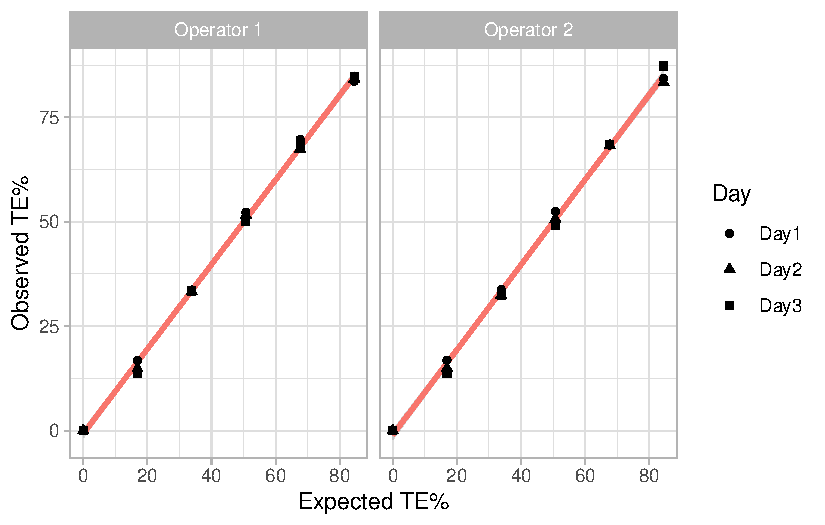
\includegraphics{index_files/figure-pdf/fig-regression-1.pdf}

}

\caption{\label{fig-regression}Linear regression of linearity samples
within each operator across the three days.}

\end{figure}%

\textsubscript{Source:
\href{https://jinkaiteo.github.io/quarto-template/index.qmd.html}{Article
Notebook}}

\section{Conclusion}\label{conclusion}

The data from this set of data support the claim of linearity of the
Transduction Efficiency (TE) Assay over the range from 0 to 80\% TE.

\section*{References}\label{references}
\addcontentsline{toc}{section}{References}

\phantomsection\label{refs}
\begin{CSLReferences}{1}{0}
\vspace{1em}

\bibitem[\citeproctext]{ref-rmarkdown2023}
Allaire, J., Xie, Y., Dervieux, C., McPherson, J., Luraschi, J., Ushey,
K., et al. (2023). \emph{{rmarkdown}: Dynamic documents for r}.
Retrieved from \url{https://github.com/rstudio/rmarkdown}

\bibitem[\citeproctext]{ref-Borman_Elder_2017}
Borman, P., \& Elder, D. (2017). Q2(R1) validation of analytical
procedures. \emph{ICH Quality Guidelines}, 127--166.
\url{https://doi.org/10.1002/9781118971147.ch5}

\bibitem[\citeproctext]{ref-webshot2}
Chang, W. (2023). \emph{webshot2: Take screenshots of web pages}.
Retrieved from \url{https://CRAN.R-project.org/package=webshot2}

\bibitem[\citeproctext]{ref-flextable}
Gohel, D., \& Skintzos, P. (2024). \emph{{flextable}: Functions for
tabular reporting}. Retrieved from
\url{https://CRAN.R-project.org/package=flextable}

\bibitem[\citeproctext]{ref-huxtable}
Hugh-Jones, D. (2024). \emph{{huxtable}: Easily create and style tables
for LaTeX, HTML and other formats}. Retrieved from
\url{https://CRAN.R-project.org/package=huxtable}

\bibitem[\citeproctext]{ref-jtools}
Long, J. A. (2022). \emph{{jtools}: Analysis and presentation of social
scientific data}. Retrieved from
\url{https://cran.r-project.org/package=jtools}

\bibitem[\citeproctext]{ref-base}
R Core Team. (2023). \emph{{R}: A language and environment for
statistical computing}. Vienna, Austria: R Foundation for Statistical
Computing. Retrieved from \url{https://www.R-project.org/}

\bibitem[\citeproctext]{ref-tidyverse}
Wickham, H., Averick, M., Bryan, J., Chang, W., McGowan, L. D.,
François, R., et al. (2019). Welcome to the {tidyverse}. \emph{Journal
of Open Source Software}, \emph{4}(43), 1686.
\url{https://doi.org/10.21105/joss.01686}

\bibitem[\citeproctext]{ref-rmarkdown2018}
Xie, Y., Allaire, J. J., \& Grolemund, G. (2018). \emph{R markdown: The
definitive guide}. Boca Raton, Florida: Chapman; Hall/CRC. Retrieved
from \url{https://bookdown.org/yihui/rmarkdown}

\bibitem[\citeproctext]{ref-rmarkdown2020}
Xie, Y., Dervieux, C., \& Riederer, E. (2020). \emph{R markdown
cookbook}. Boca Raton, Florida: Chapman; Hall/CRC. Retrieved from
\url{https://bookdown.org/yihui/rmarkdown-cookbook}

\bibitem[\citeproctext]{ref-kableExtra}
Zhu, H. (2024). \emph{{kableExtra}: Construct complex table with
{``{kable}''} and pipe syntax}. Retrieved from
\url{https://CRAN.R-project.org/package=kableExtra}

\end{CSLReferences}



\end{document}
